%!TEX root = ../username.tex
\chapter{The Software}
\hspace*{-0.15cm}To bring everything together, this chapter will cover how the application was created using JUCE. It will begin with a description of the data structures that were used before describing their implementation. Then, the process of creating the user interface will be described. Finally, it will end with how the software runs under several different host applications.
\section{Data Structures and Implementation}
Both Comb Filters and Allpass Filters use a queue ADT for their implementation. However, they rely on an implementation that uses a \textit{circular array} so that audio data can be continuously fed into the application. In other words, an array with modular arithmetic is used so that audio data can be continuously queued. This ignores the usual problem that come from circular arrays; that current lengths can be ambiguous for the same \textit{front} and \textit{back} pointer \cite{carrano2016data}. For the purposes that this data structure is being used for for, all that matters is that data can be continuously processed in the system and overwritten when new data comes in.

To implement a Comb Filter, one can imagine an array of floats representing a buffer of data to be processed. A subsection of this buffer will be specified as the signal to repeat of an arbitrary length. This is the delay buffer. To match the behavior expected of a Comb Filter in code, one can imagine filling a temporary buffer with data. One can then read this data back to the original buffer once it has been processed (i.e., the write pointer of the circular array has moved past the data read thus far). JUCE provides a datatype \verb|AudioBuffer<Type>| that allows the programmer to copy data from one buffer to the next (or rather, the primary buffer to output and a buffer containing the temporary delayed signal) - however, it is up to the programmer to implement the circular behavior themselves so that undefined behavior does not occur.
\lstset{language =[ANSI]C++}
\lstset{backgroundcolor=\color{white},rulecolor=\color{black}}
\lstset{linewidth=.95\textwidth,breaklines=true}
\lstset{commentstyle=\textit,stringstyle=\upshape,showspaces=false}
\lstset{frame = single}
\lstset{numbers=left,numberstyle=\tiny,basicstyle=\small}
\lstset{commentstyle=\normalfont\itshape,breakautoindent=true}
\lstset{abovecaptionskip=1.2\baselineskip,xleftmargin=30pt}
\lstset{framesep=6pt}
\begin{singlespace}
\lstinputlisting[caption=The high level code of a Comb Filter., label=motion]{source/pseudo1.txt}
\end{singlespace} \hfill \break
\hspace*{0.6cm}This circular behavior can be defined as a custom class \verb|DelayLine|, whose members are defined in Listing A.1. As part of this class, to implement \verb|fillBuffer()|, JUCE provides functions under the \verb|juce_audio_basics/juce_audio_basics.h| header. These include the functions \verb|getNumSamples()|, \verb|copyFrom()|, and \verb|getWritePointer()|. Essentially, the function \verb|fillBuffer()| first checks the size of the delay buffer. Upon doing so, if the write position (the \textit{front} pointer of the circular array) is within the bounds of the delay buffer, then the audio data can simply be copied from the delay buffer to the buffer via the \verb|copyFrom()| function. If not, care is taken to calculate the correct length of the delay buffer and how many samples are present between the \textit{head} and the \textit{back} pointer of the delay line. The \verb|copyFrom()| function can then be used in a similar manner.

This takes care of filling the buffer with the data sent through the delay line (Figure 4.3, filling the buffer with the delay of time \textit{T}). However, \verb|readFromBuffer()| must read this data to be sent back through the filter as an input with some gain \textit{g}. To calculate the gain parameter, the naive approach would be to set the variable to some constant. However, this does not work as the length of the decay would be different for each delay time \textit{T}. To ensure that each delay line does not have different lengths, \textit{g} be calculated as a function with respect to the length of time that the programmer wishes to have the Comb Filter last. This can be done with the following equation:

\begin{center}
\scalebox{1.3}{
$
g = 10^{\frac{-3DT_s}{RT_{60}}}
$
}
\end{center}

where $D$ is the delay line length in seconds, $T_s$ the sample rate, and $RT_{60}$ the reverberation time in seconds  \cite{pirkle2019designing}. However, one can simplify this further as the sample rate conversion is simply an intermediary to convert seconds to discrete buffers. If working purely with lengths of buffers, this simplifies to:

\begin{center}
\scalebox{1.3}{
$
g = 10^{\frac{-3D_b}{RT_b}}
$
}
\end{center}

where $D_b$ is the delay line length in buffers and $RT_b$ is likewise the $RT_{60}$ time in buffers. This translates to the following code:

\begin{singlespace}
\lstinputlisting[caption=Code to calculate $g$ within a delay line., label=motion]{source/pseudo2.txt}
\end{singlespace} \hfill \break
\hspace*{0.6cm}It is worth reiterating, the gain \textit{g} applied during the \verb|readFromBuffer()| step \textit{must} be calculated for each different delay length. For multiple delays, if a constant \textit{g} is applied for each different delay length, the comb filters will finish decaying at different points in time. This calculation avoids this. The function separates this approach from being just a number of delays played at once - they all contain the same $RT_{60}$ time, despite being of different delay lengths with each repeated signal.

With the gain parameter handled, the \verb|readFromBuffer()| function can be implemented by adding the delayed signal back to the input buffer with the calculated gain applied. This is different from the copy step as the signal is not being replaced - the new signal must be the sum of the next incoming signal with the (now delayed) previous. JUCE contains the function \verb|addFromWithRamp()| that accomplishes this.

\begin{singlespace}
\lstinputlisting[caption=Code to take the sum of two signals., label=motion]{source/pseudo3.txt}
\end{singlespace} \hfill \break
\hspace*{0.6cm}Lastly, it is the responsibility of the programmer to update the \textit{head} pointer to ensure that the circular buffer stays within its intended space in memory and prevents undefined behavior from occuring.

\begin{singlespace}
\lstinputlisting[caption=Code to implement circular behavior in an array., label=motion]{source/pseudo4.txt}
\end{singlespace} \hfill \break
\hspace*{0.6cm}Placing each component in context, these functions work together by being called within a greater \verb|processBlock()| function that takes a buffer, applies some processing, and returns the buffer back to the DAW. This function is run every time a buffer is sent from the DAW to the VST application. As mentioned in Chapter 3, there is only so much time for processing to be completed, so code must be efficient enough to avoid dropped buffers. The code within \verb|processBlock()| begins by checking how many channels are being processed within the buffer. Most cases, this number is either \textit{mono} (1 channel) or \textit{stereo} (2 channels). Upon determining the correct number of channels, the program then iterates through a \textit{for} loop to process the audio data for each channel. Here, one can begin by making a temporary copy of the buffer to process (allowing the programmer to make a separate \textit{wet} and \textit{dry} mix). This temporary buffer is then sent to a custom class \verb|TestReverb| that processes the buffer through the custom function \verb|processReverb()|. Here, the signal is separated into four separate channels - or, Comb Filters, rather - and processes the audio in the same manner done in Listing 6.1. Each channel of audio is then summed back with the original temporary buffer using JUCE's \verb|addFrom()| function. The programmer can specify any number of Comb Filters in parallel during this step. In a similar manner, Allpass Filters can be implemented by applying a gain of $1 - g^2$ to the signal (post-Comb Filter) that is summed with the inverse of the signal $-g$ prior to the Comb Filter being applied. Upon processing being completed, the function updating the \textit{head} pointer can be called, and the program is ready to recieve the next buffer from the DAW.

Convolution reverbs can be implemented using a similar approach, but can be aided through the use of JUCE's DSP class. [].


Through these filters, Schroeder's design can be implemented in code. Should the user wish to manipulate parameters in real-time, however, additional functionality must be implemented.

\section{User Interface}
As previously discussed in Chapter 3, the structure of an audio plugin mandates that the user interface and backend processing are separated. While the code mentioned previously handles the back end processing, it is up to the programmer to handle how the user interface functions so that the user can specify various parameters of the plugin without modifying the code manually. This allows the user to specify items such as room size, gain, and wet/dry mix.

To do this, private members can be added to the \verb|PluginEditor| class and \verb|PluginProcessor| class respectively. Private members in the \verb|PluginEditor| class handle the specific frontend objects - that is, the sliders, knobs, and menu items themselves. Listing 6.5 describes how one such UI element can be implemented from the class constructor.

\begin{singlespace}
\lstinputlisting[caption=Code to create a UI element., label=motion]{source/pseudo5.txt}
\end{singlespace} \hfill \break
\hspace*{0.6cm}However, this does not take into account how the two threads communicate with one another. To do this, JUCE contains a \verb|private juce::Slider::Listener| object under the \verb|juce_gui_basics/juce_gui_basics.h| header that allows the program to track the current value of the user interface. Upon doing so, the GUI updates the state of the corresponding \verb|PluginProcessor| value to align with the frontend.

\begin{singlespace}
\lstinputlisting[caption=Code to update backend parameters., label=motion]{source/pseudo6.txt}
\end{singlespace} \hfill \break
\hspace*{0.6cm} Through these principles, multiple UI elements can be added that allow the programmer to update any parameter in real time.

\section{Compatibility with DAWs}
Testing the plugin on Debian GNU/Linux 12, it is verified working on DAWs such as Reaper and Renoise. It is expected to work on Windows as well, but may require additional code signing to compile in Mac OSX without enabling developer mode.

\begin{figure}[h] % [h] used to prevent {figure} from doing weird positioning
	\begin{center}
		\fbox{
		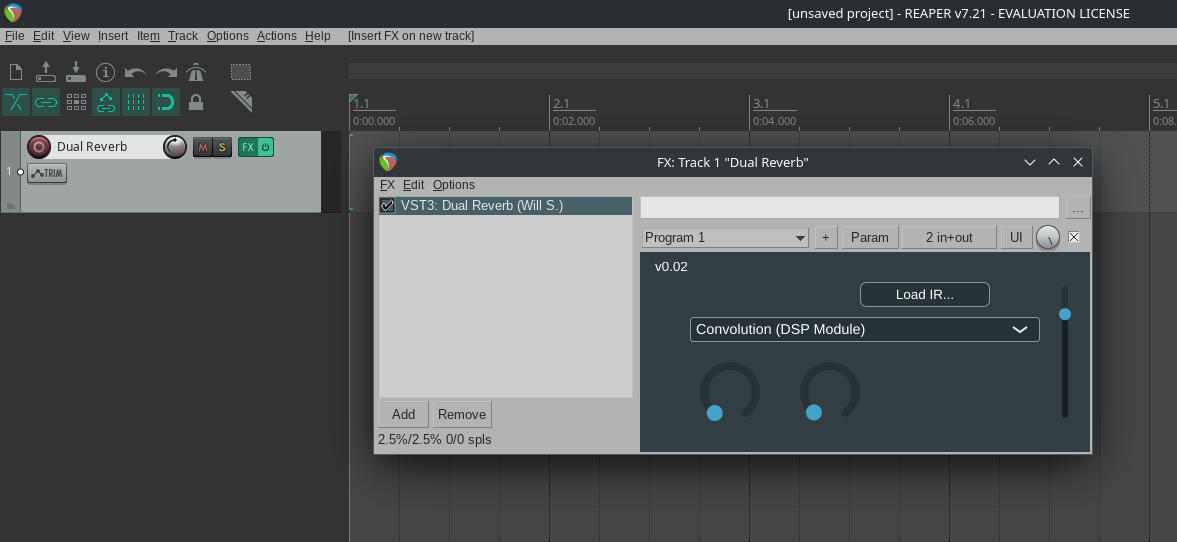
\includegraphics[width=14cm]{figures/DAW-1.png}
		}
		\caption{The reverb plugin running within Reaper.}
	\end{center}
\end{figure}

\begin{figure}[h] % [h] used to prevent {figure} from doing weird positioning
	\begin{center}
		\fbox{
		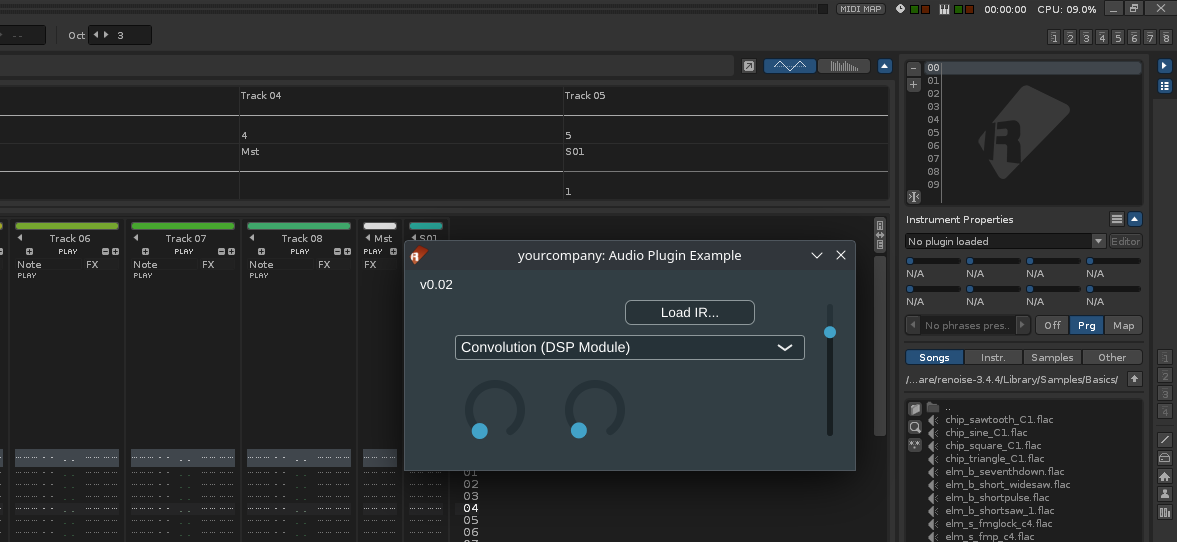
\includegraphics[width=14cm]{figures/DAW-2.png}
		}
		\caption{The reverb plugin running within Renoise.}
	\end{center}
\end{figure}
